\documentclass[a4paper]{article}
\usepackage[UKenglish]{babel}

\usepackage{preamble}
\usepackage{cancel}

\usepackage{graphicx}
\graphicspath{ {./imgs/} }

\title{MA146 Methods of Mathematical Modelling 1, Assignment 4}
\author{Dyson Dyson}
\date{}

\begin{document}

\maketitle

\setlength{\parindent}{0em}
\setlength{\parskip}{1em}

\question{2}

$$\diff t v(t) = -v(t) + \varepsilon v(t)^2, \quad t > 0, \quad v(0) = 1$$

\subsection{~}

I have no idea what substitution to use, sorry.

\subsection{~}

Consider $v(t) = v_0(t) + \varepsilon v_1(t)$. Then \begin{align*}
	\diff t v(t) &= \diff t v_0(t) + \varepsilon \diff t v_1(t)\\[1ex]
				 &= -v_0(t) - \varepsilon v_1(t) + \varepsilon \l(v_0(t)^2 + 2 \varepsilon v_0(t) v_1(t) + \varepsilon^2 v_1(t)^2 \r)\\[1ex]
				 &= -v_0(t) - \varepsilon v_1(t) + \varepsilon v_0(t)^2 + \cancelto{0}{\varepsilon^2 \l(\cdots\r)}\\[1ex]
	\therefore \diff t v_0(t) + \varepsilon \diff t v_1(t) &= -v_0(t) - \varepsilon v_1(t) + \varepsilon v_0(t)^2
\end{align*}

And the initial condition becomes $v_0(0) + \varepsilon v_1(0) = 1$. Unfortunately, I have no idea where to go from here.

\question{3}

\subsection{~}

$$3\text{K} + 4\text{M} \xrightleftharpoons[\ r_2\ ]{\ r_1\ } 2\text{A} + 6\text{B}$$

Let $k(t)$ be the concentration of K and likewise pairing $m(t)$ with M, $a(t)$ with A, and $b(t)$ with B. Then we get the following equations \begin{align*}
	\diff t k(t) &= -3 r_1 k(t) m(t) + 3 r_2 a(t) b(t)\\[1ex]
	\diff t m(t) &= -4 r_1 k(t) m(t) + 4 r_2 a(t) b(t)\\[1ex]
	\diff t a(t) &= 2 r_1 k(t) m(t) - 2 r_2 a(t) b(t)\\[1ex]
	\diff t b(t) &= 6 r_1 k(t) m(t) - 6 r_2 a(t) b(t)
\end{align*}

\subsection{~}

$$2\text{NOCl} \xrightarrow{\ k\ } 2\text{NO} + \text{Cl}_2$$

Let $s(t)$ be the concentration of nitrosyl chloride, $n(t)$ be the concentration of nitric oxide, and $c(t)$ be the concentration of chlorine. Then the rate equations are \begin{align*}
	\diff t s(t) &= -2ks(t)\\[1ex]
	\diff t n(t) &= 2ks(t)\\[1ex]
	\diff t c(t) &= ks(t)
\end{align*}

\subsection{~}

$$S + I \xrightarrow{\ \beta\ } I \xrightarrow{\ \gamma\ } R$$

\question{4}

\subsection{~}

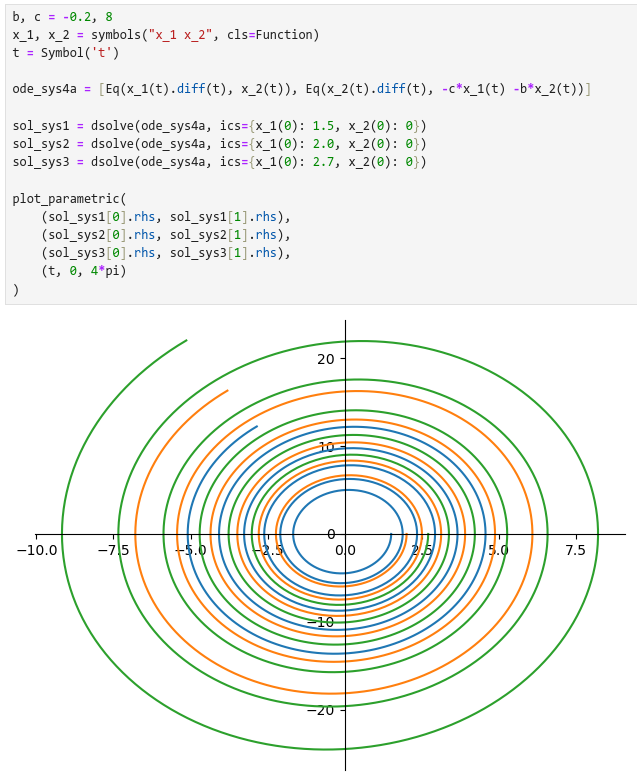
\includegraphics[scale=0.55]{Q4}

\subsection{~}

Assignment 1 question 2 was about the differential equation $$a \f{\d^2}{\d t^2}x(t) + b \diff t x(t) + cx(t) = 0$$

The system \begin{align*}
	x_1'(t) &= x_2(t)\\[1ex]
	x_2'(t) &= -c x_1(t) - b x_2(t)
\end{align*}is related in that we can imagine $x_1(t) = x(t)$ and $\ds x_2(t) = \diff t x(t)$. Then the system becomes \begin{align*}
	\diff t x(t)          &= \diff t x(t)\\[1ex]
	\f{\d^2}{\d t^2} x(t) &= -c x(t) - b \diff t x(t)
\end{align*}

The first line is just obviously always true, and the second line is equivalent to the differential equation given in assignment 1 question 2, just with $b$ and $c$ scaled to make $a=1$.

\end{document}
